\section{Background}\label{sec:background}

\subsection{Mixed Integer Linear Programming (MILP) Problems}\label{subsec:mixed-integer-linear-programming-(milp)-problems}


These problems are linear optimization problems where some of the decision variables are integers, and some are continuous.
It is possible to formulate MILP problems as follows:

\begin{equation}
    \begin{aligned}
        \text{minimize} \quad & \textbf{c}^T \textbf{x} \\
        \text{s.t.} \quad & \textbf{A}\textbf{x} \leq \textbf{b} \\
        & \textbf{x} \in \mathbb{Z}^p \times \mathbb{R}^{n-p}\\
    \end{aligned}\label{eq:equation}
\end{equation}


where \textbf{c} \begin{math} \in \mathbb{R}^n \end{math} represents the objective coefficient vector, \textbf{A} \begin{math} \in \mathbb{R}^{mxn} \end{math} represents the constraint coefficient matrix,  represents the right-hand-side vector, and  p \begin{math} \leq \end{math} n indicates the number of integer variables.
MILP problems are usually solved by Branch \& Bound algorithm.


\subsection{The LP Relaxation of a MILP Problem}\label{subsec:the-lp-relaxation-of-a-milp-problem}


LP Relaxation of a MILP problem is the problem obtained by ignoring the integrality conditions on the variables in the MILP problem as follows:

\begin{equation}
    \begin{aligned}
        \text{minimize} \quad & \textbf{c}^T \textbf{x} \\
        \text{s.t.} \quad & \textbf{A}\textbf{x} \leq \textbf{b} \\
        & \textbf{x} \in \mathbb{R}^{n}\\
    \end{aligned}\label{eq:equation}
\end{equation}


It is possible to solve this form of the problem using Linear Programming (LP) techniques such as Simplex algorithm.


\subsection{Bipartite Graph Representation of a MILP Problem}
\label{sec:bipartite_graph_representation}


To employ GNN techniques, such as GCNN and GAT, in tackling Combinatorial Optimization problems, these problems need to be represented as graphs.
Combinatorial Optimization problems can be represented as bipartite graphs.
The nodes on the left side of the bipartite graph represent the constraints in the MILP problem, with each constraint corresponding to a node.
The nodes on the right side of the bipartite graph represent the variables in the MILP problem, with each variable corresponding to a node.
If a variable is part of a constraint, there is an undirected edge between the corresponding nodes.
The coefficient of the variable in the constraint is a feature of the corresponding edge.
Figure 2.1 illustrates the bipartite graph representation of a MILP problem with 3 variables and 2 constraints.

This is an example on how to add a figure.
The figure is shown in Figure~\ref{fig:biparite-graph}.

\begin{figure}[htb!]
    \centering
    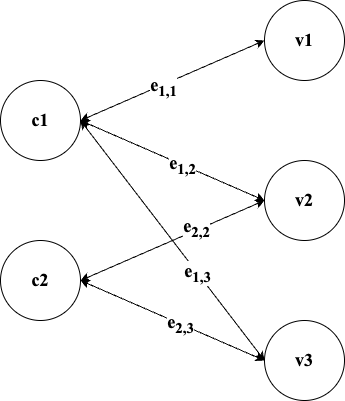
\includegraphics[width=0.45\textwidth]{figures/Bipartite Graph.drawio}
    \caption{Bipartite graph representation of a MILP problem with n = 3 variables and m = 2 constraints. If a variable is part of a constraint, there is an undirected edge between the corresponding nodes.}
    \label{fig:biparite-graph}
\end{figure}